% You should title the file with a .tex extension (hw1.tex, for example)
\documentclass[a4paper, 11pt]{article}

\usepackage{amsmath}
\usepackage{amssymb}
\usepackage{fancyhdr}
\usepackage{graphicx}

\usepackage[margin=1in]{geometry}

\newcommand{\question}[2] {\vspace{.25in} \hrule\vspace{0.5em}
\noindent{\bf #1: #2} \vspace{0.5em}
\hrule \vspace{.10in}}
\renewcommand{\part}[1] {\vspace{.10in} {\bf (#1)}}

\newcommand{\myname}{Natthakan Euaumpon}
\newcommand{\myemail}{natthakaneuaumpon@gmail.com}
\newcommand{\myhwnum}{2}

\setlength{\parindent}{0pt}
\setlength{\parskip}{5pt plus 1pt}
 
\pagestyle{fancyplain}
\lhead{\fancyplain{}{\textbf{HW\myhwnum}}}      % Note the different brackets!
\rhead{\fancyplain{}{\myname\\ \myemail}}
\chead{\fancyplain{}{ICCS310 }}

\begin{document}

\medskip                        % Skip a "medium" amount of space
                                % (latex determines what medium is)
                                % Also try: \bigskip, \littleskip

\thispagestyle{plain}
\begin{center}                  % Center the following lines
{\Large ICCS310: Assignment \myhwnum} \\
\myname \\
\myemail \\
January 2020 \\
\end{center}

\question{1}{Regex to NFA/DFA}
\part{1}\\
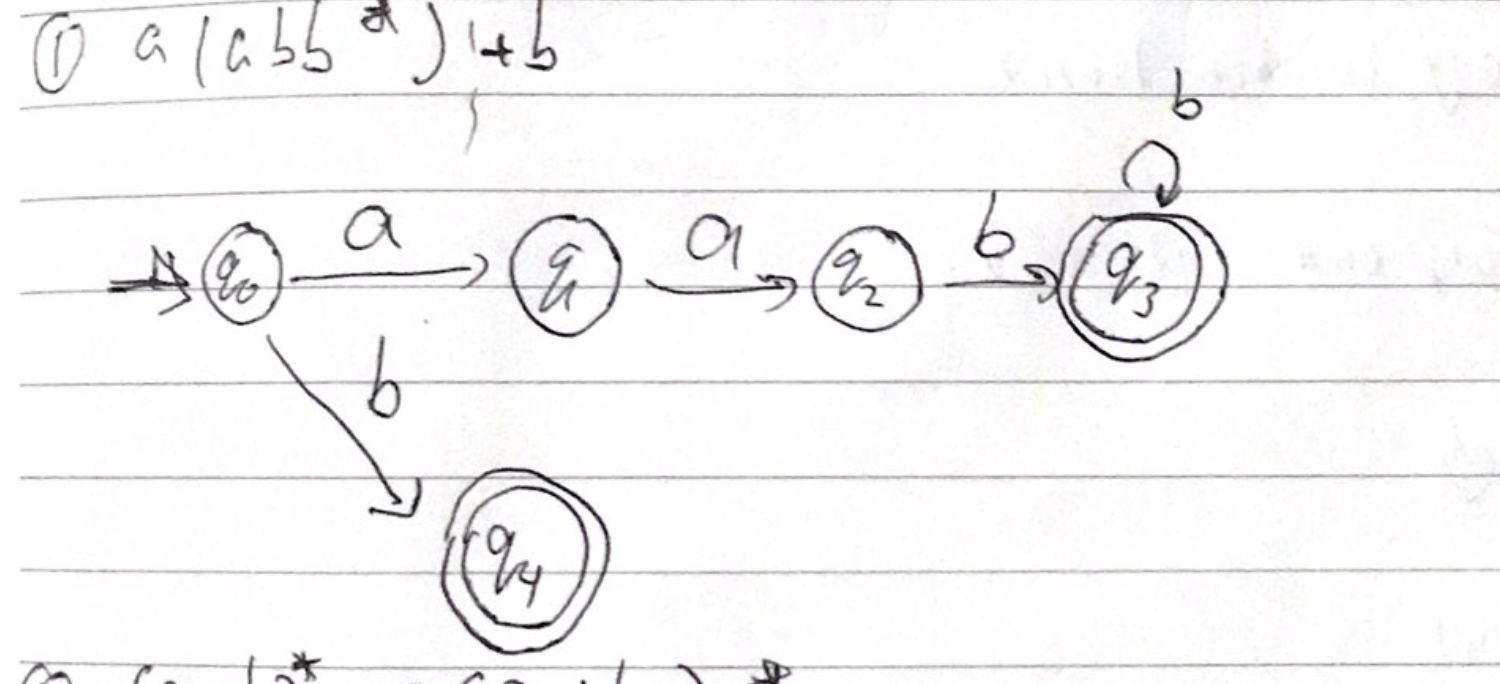
\includegraphics[width=\textwidth]{Q1-1.png}\\
\part{2}\\
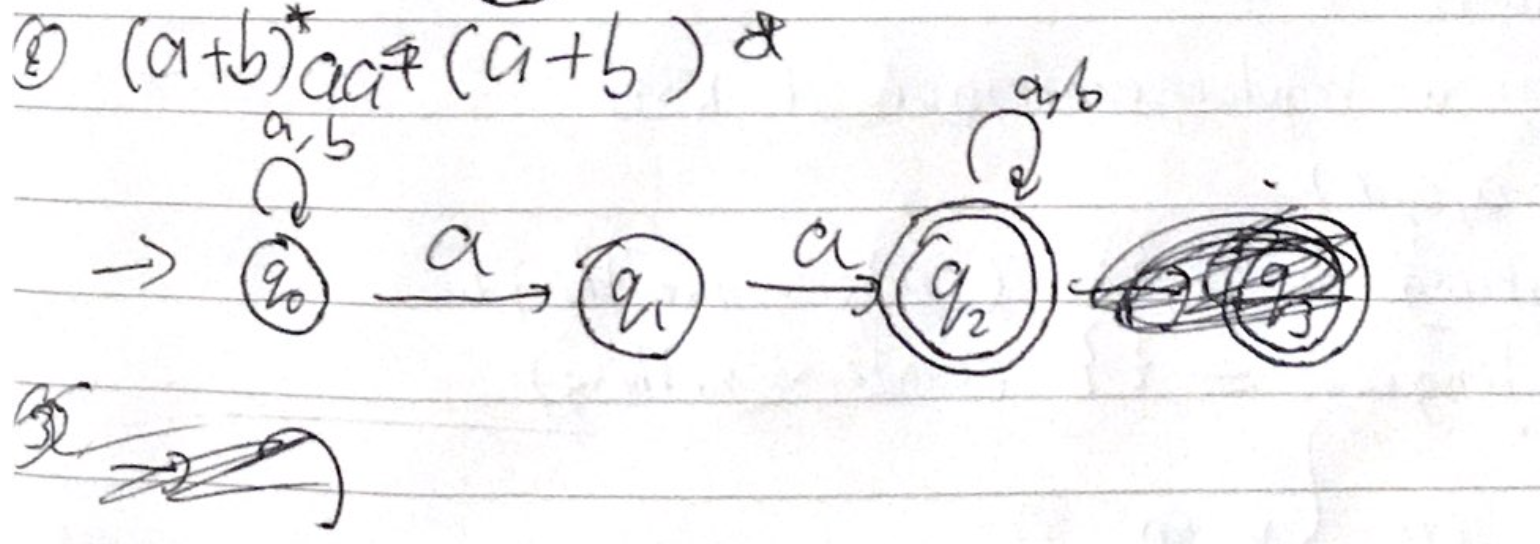
\includegraphics[width=\textwidth]{Q1-2.png}\\
\part{3}\\
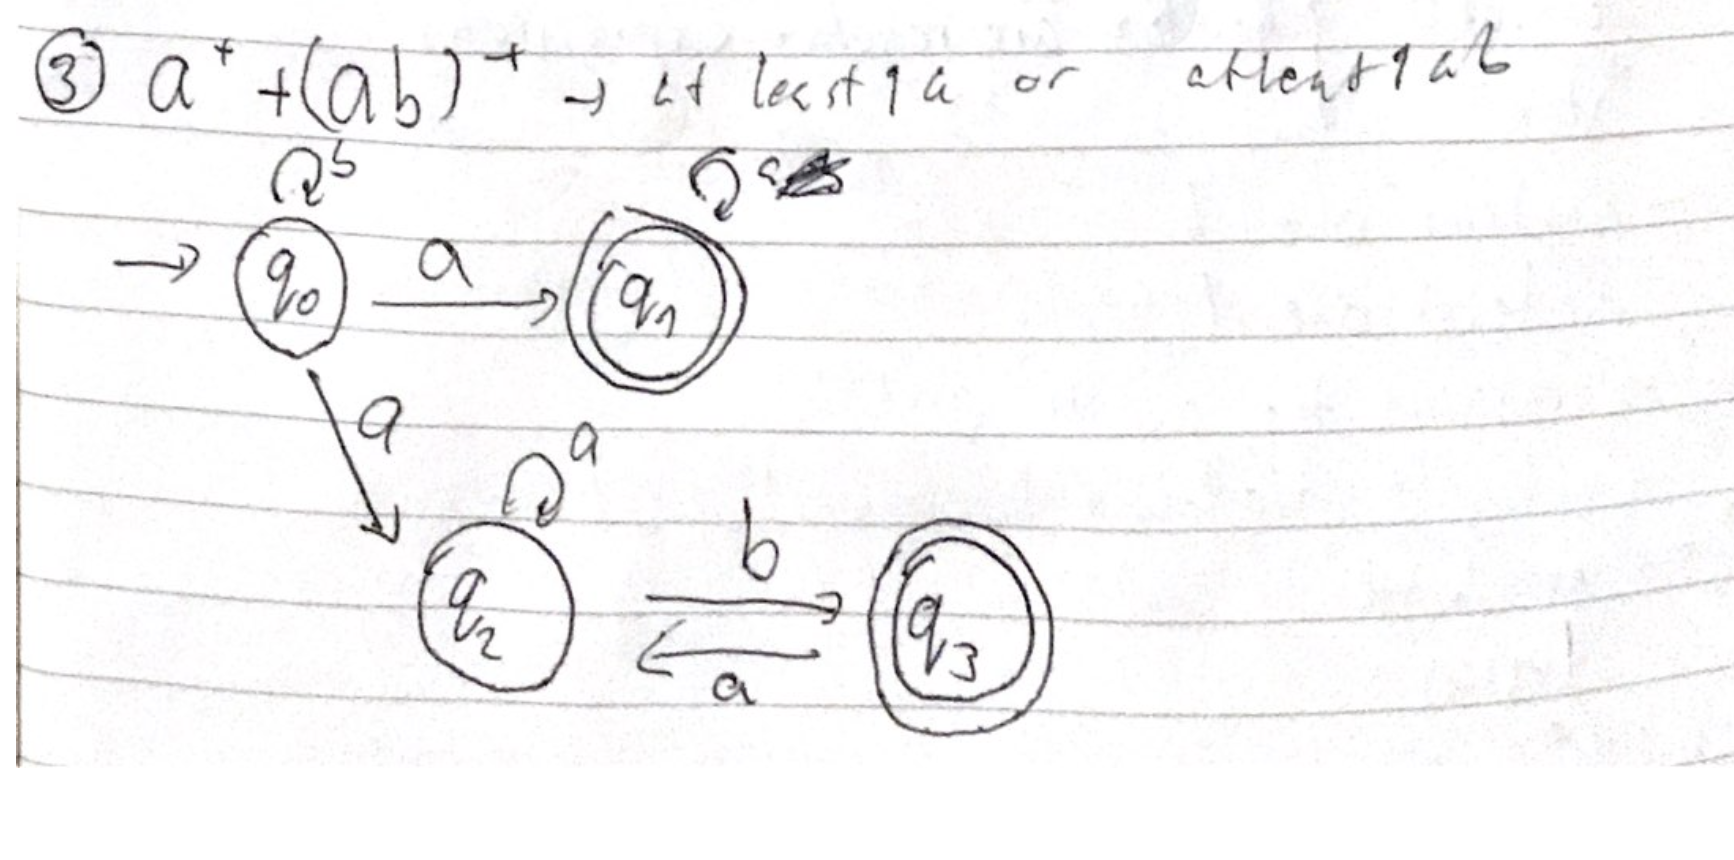
\includegraphics[width=\textwidth]{Q1-3.png}

\question{2}{Finite-State Machines to Regex}
\part{1}\\
$\emptyset^*$\\
\part{2}\\
$a^* + a^*b^+a^+b$

\question{3}{Binary Addition}
We already proof in class that if L is regular language than $L^R$ is also a regular language. When we add a binary number we start by adding the rightmost bit and in every step of binary addition there is a carry bit which will go to the next step. This carry bit can be either 0 or 1. We will construct a machine that will recognise $A^R$. This machines will perform the addition of the first two row. In each step the machine will check if the result is equal to the  third row or not. We use the states of the machine to remember the carry bit. We can define a function as:\\
$0 + 0 = 0$\\
$0 + 1 = 1$\\
$1 + 0 = 1$\\
$1 + 1 = 0$\\
We will also have a function that tell us what is the carry bit when we sum the 3 bits together.The machine will have 2 states $q_0$ and $ q_1$ which will represent the carry bit ($q_0$ for 0 and $q_1$ for 1). Where $q_0$ is both starting state and accepting state because the carry digit need to be zero when the addition is complete. This mean the machine will accept only when the sum of the first 2 row and the carry bit is equal to the third row and that the carry bit is zero.

\question{4}{Division Operation?}
If $L_1$ and $L_2$ are regular then their should be a DFA for both $L_1$ and $L_2$.  Then we can construct a DFA $L_1 = L(M)$. Let the DFA be $M = (Q,\Sigma,\delta,q_0,F)$. We will construct another DFA that will run with the first DFA. Let it be $\hat{M} = (Q,\Sigma,\delta,q_0,\hat{F})$. For each node, if there is a walk from that node to the final node using a string in $L_2$ then put that node in $\hat{F}$. After looking through every $q_i$ we have constructed $\hat{M}$. Now we have 2 DFA. Let k be an element in $L_1/L_2$. Then there should be $k \in L_2$ such that $a \cdot k \in L_1$. This indicate that $\delta^*(q_0,a \cdot k) \in F$. So there must be an element $b \in Q$ such that $\delta^*(q_0, k) = b$ and $\delta^*(b, a) \in F$. We already show that $\hat{M}$ accept k. This implies that $a \in L_2$. So $a \cdot k \in L_1$ and that $L_1/L_2$ is regular.

\question{5}{Does It Accept Everything?}
If we minimize a DFA using regular expression and the it's left with only accepting state then the DFA accept everything. This is because 


\end{document}

